% ============================================================================
% MADHAV'S CONTRIBUTION: Experimental Manipulation Results
% To be inserted in Section 4 after "Elicitation Invariance"
% ============================================================================

\textbf{Model Choice vs Expert Persona Variance}

We tested whether expert persona or model choice drives forecast variance using Fréchet ANOVA on Beta distributions fit to elicited percentiles (p25, p50, p75) via least squares (rejecting fits where $|\text{CDF}(p_q) - q| > 0.05$). Three models (Claude Sonnet 4.5, GPT-4o, Gemini 2.5 Pro), 10 personas, 10 runs per persona, tested on three attack steps: TA0002 (50\% baseline), TA0007 (85\% baseline), T1657 (30\% baseline), all using Imaginairy benchmark (difficulty=22, CVSS=7.5).

\textit{Within-model persona tests:} Claude and GPT-4o showed no significant persona effects (ICC\_F 5.7--13.9\%, all $p > 0.05$). Gemini showed two significant effects at TA0002 and TA0007 (ICC\_F 18.3--24.9\%, $p < 0.05$) but remained smaller than cross-model effects (Table~\ref{tab:persona_variance}).

\textit{Cross-model tests:} Model choice explained 48--69\% of distributional variance (all $p < 0.001$, Table~\ref{tab:model_variance}), 3.5--12$\times$ more than persona. Figures~\ref{fig:persona_dist} and~\ref{fig:model_dist} show tight persona clustering within models versus clear model separation. This pattern held for both probability and quantity estimates (number of actors: model ICC\_F=24\% vs persona ICC\_F=9\%).

\begin{table}[htbp]
\centering
\caption{Within-model persona variance (Fréchet ANOVA). No significant effects for Claude/GPT-4o. Gemini shows limited variation.}
\label{tab:persona_variance}
\small
\begin{tabular}{llcccc}
\toprule
\textbf{Model} & \textbf{Step} & \textbf{N} & \textbf{T$_n$} & \textbf{p} & \textbf{ICC\_F} \\
\midrule
Claude Sonnet 4.5 & TA0002 (50\%) & 100 & 0.008 & 0.400 & 9.6\% \\
 & TA0007 (85\%) & 80 & 0.003 & 0.195 & 13.9\% \\
 & T1657 (30\%) & 100 & 0.020 & 0.803 & 7.2\% \\
\midrule
GPT-4o & TA0002 (50\%) & 97 & 0.016 & 0.899 & 5.7\% \\
 & TA0007 (85\%) & 96 & 0.007 & 0.708 & 7.5\% \\
 & T1657 (30\%) & 100 & 0.043 & 0.215 & 11.8\% \\
\midrule
Gemini 2.5 Pro & TA0002 (50\%) & 88 & 0.043 & \textbf{0.030} & 18.3\% \\
 & TA0007 (85\%) & 96 & 0.007 & \textbf{0.002} & 24.9\% \\
 & T1657 (30\%) & 88 & 0.005 & 0.585 & 8.8\% \\
\bottomrule
\end{tabular}
\end{table}

\begin{table}[htbp]
\centering
\caption{Cross-model variance (Fréchet ANOVA). All steps show highly significant model effects.}
\label{tab:model_variance}
\begin{tabular}{lcccc}
\toprule
\textbf{Step} & \textbf{N} & \textbf{T$_n$} & \textbf{p-value} & \textbf{ICC\_F} \\
\midrule
TA0002 (50\%) & 285 & 0.729 & <0.001 & 55.3\% \\
TA0007 (85\%) & 272 & 0.131 & <0.001 & 48.2\% \\
T1657 (30\%) & 288 & 1.515 & <0.001 & 69.4\% \\
\bottomrule
\end{tabular}
\end{table}

\begin{figure}[htbp]
  \centering
  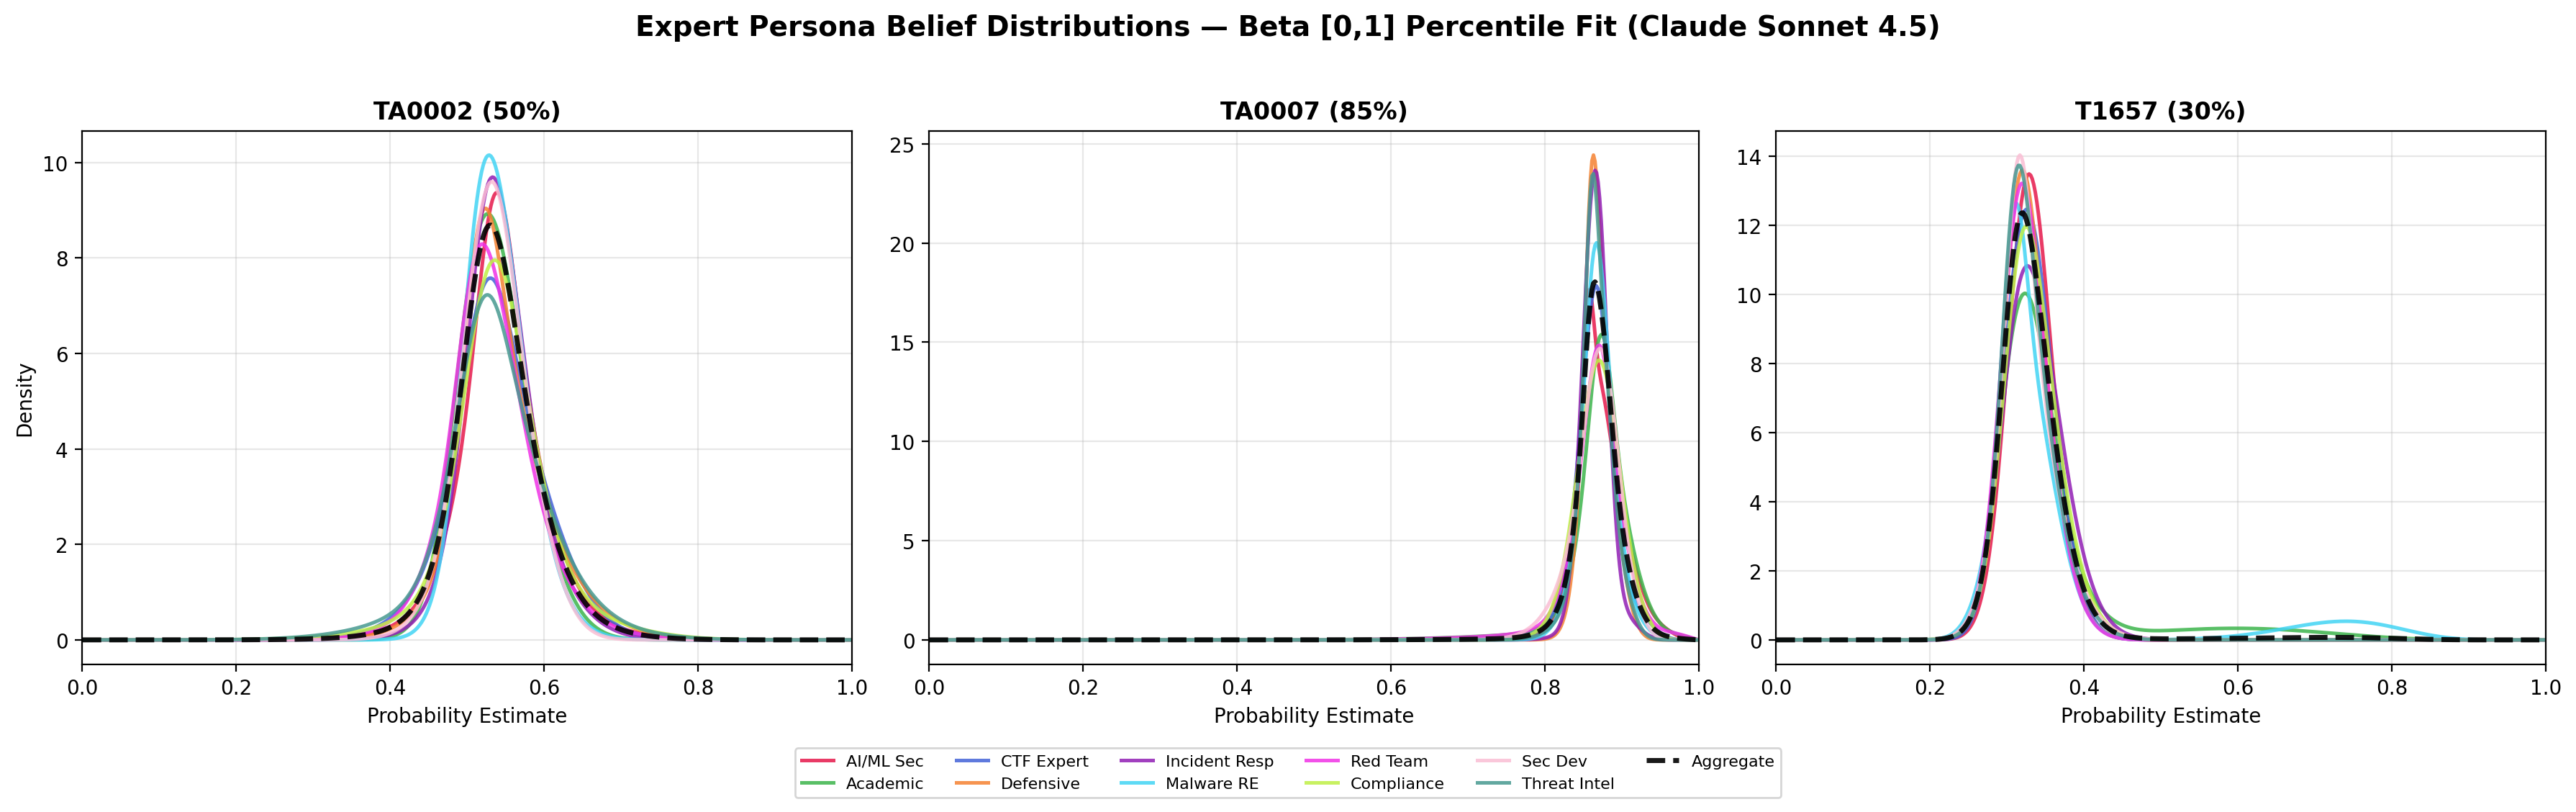
\includegraphics[width=0.85\textwidth]{figures/beta_persona_distributions_percentile_week3.png}
  \caption{Persona distributions for Claude Sonnet 4.5 overlap tightly within each attack step, consistent with minimal persona-driven variance.}
  \label{fig:persona_dist}
\end{figure}

\begin{figure}[htbp]
  \centering
  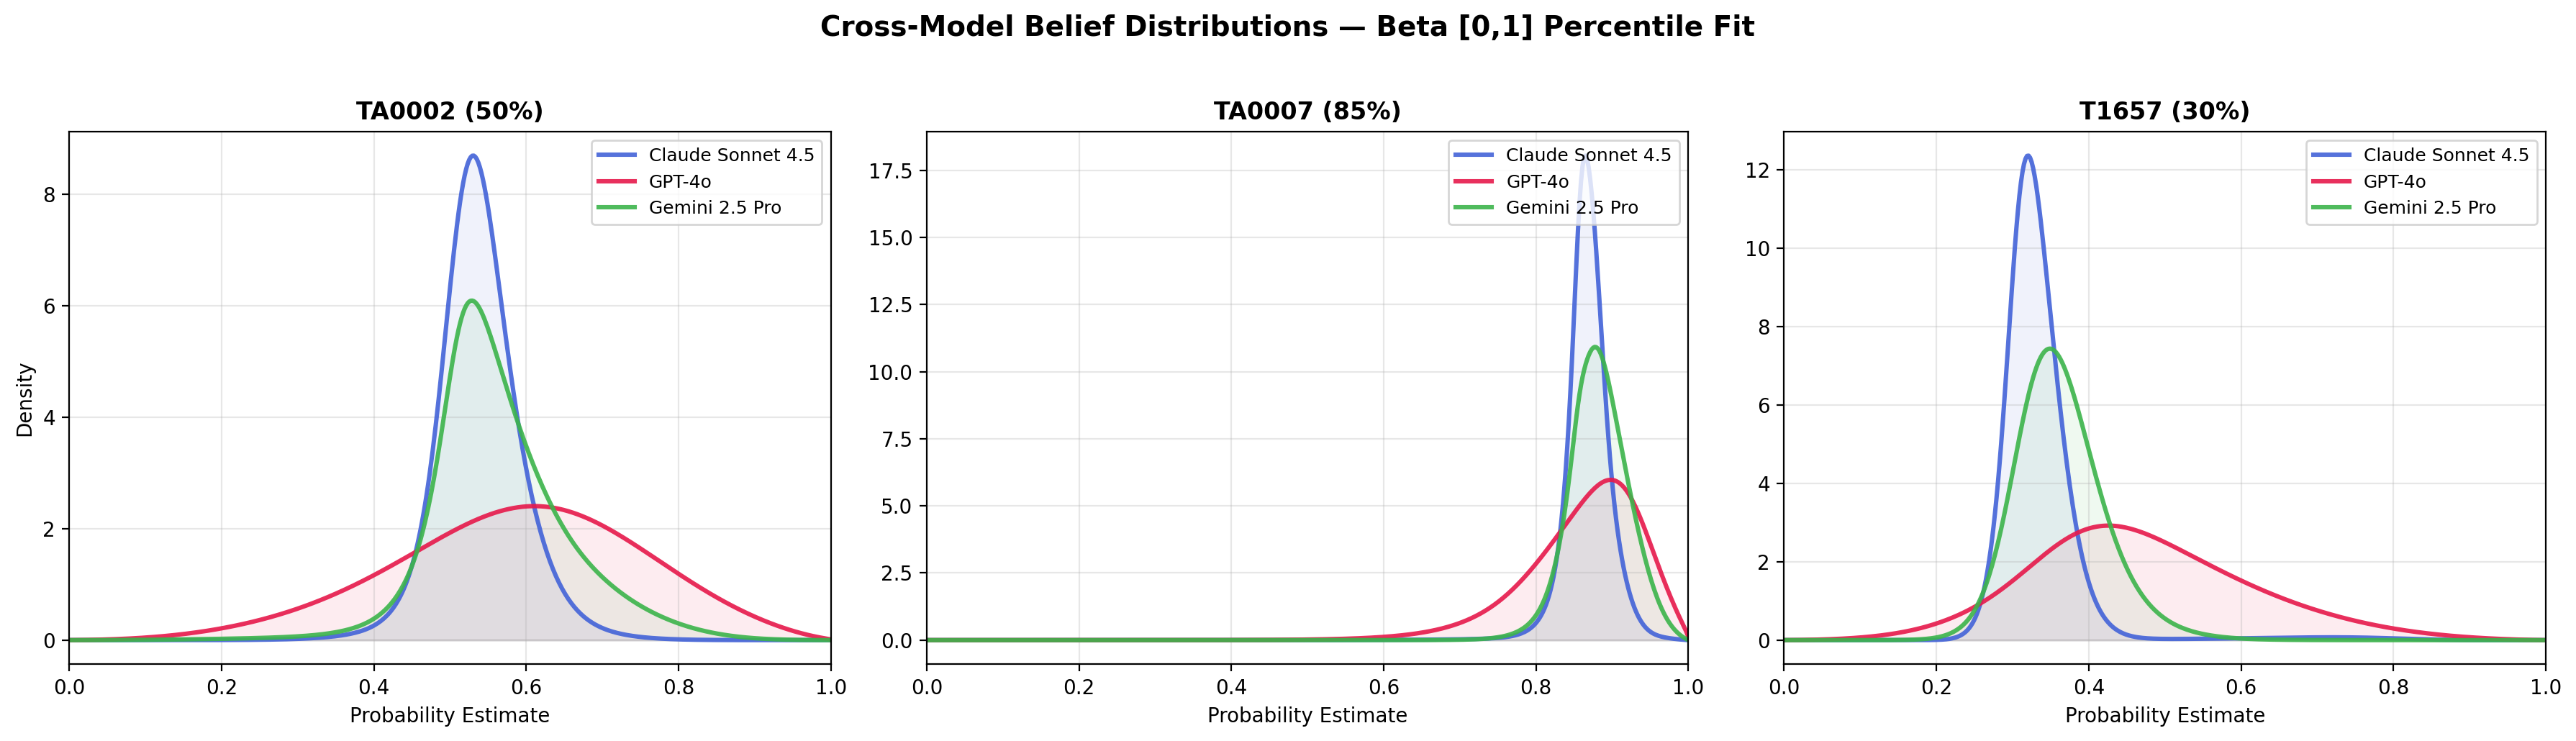
\includegraphics[width=0.85\textwidth]{figures/beta_cross_model_distributions_percentile_week3.png}
  \caption{Cross-model distributions show clear separation across all three attack steps.}
  \label{fig:model_dist}
\end{figure}

\textbf{Baseline Anchoring}

To test anchoring effects, we swept baseline probability from 10\% to 90\% (10\% increments, 10 runs per baseline) using Claude Sonnet 4.6, single persona (AI/ML Security Researcher), TA0002 (Execution step), Imaginairy benchmark. Confidence intervals removed to isolate baseline effect.

\textit{Results:} Median elicited probability tracked baseline approximately linearly (Figure~\ref{fig:baseline_uplift}), with ceiling effects at high baselines (reduced uplift near 100\%). For scenario-level quantity estimates (number of actors, unbounded), the linear relationship persisted without ceiling effects (Figure~\ref{fig:numactors_uplift}), indicating strong anchoring for both bounded and unbounded estimates.

\begin{figure}[htbp]
  \centering
  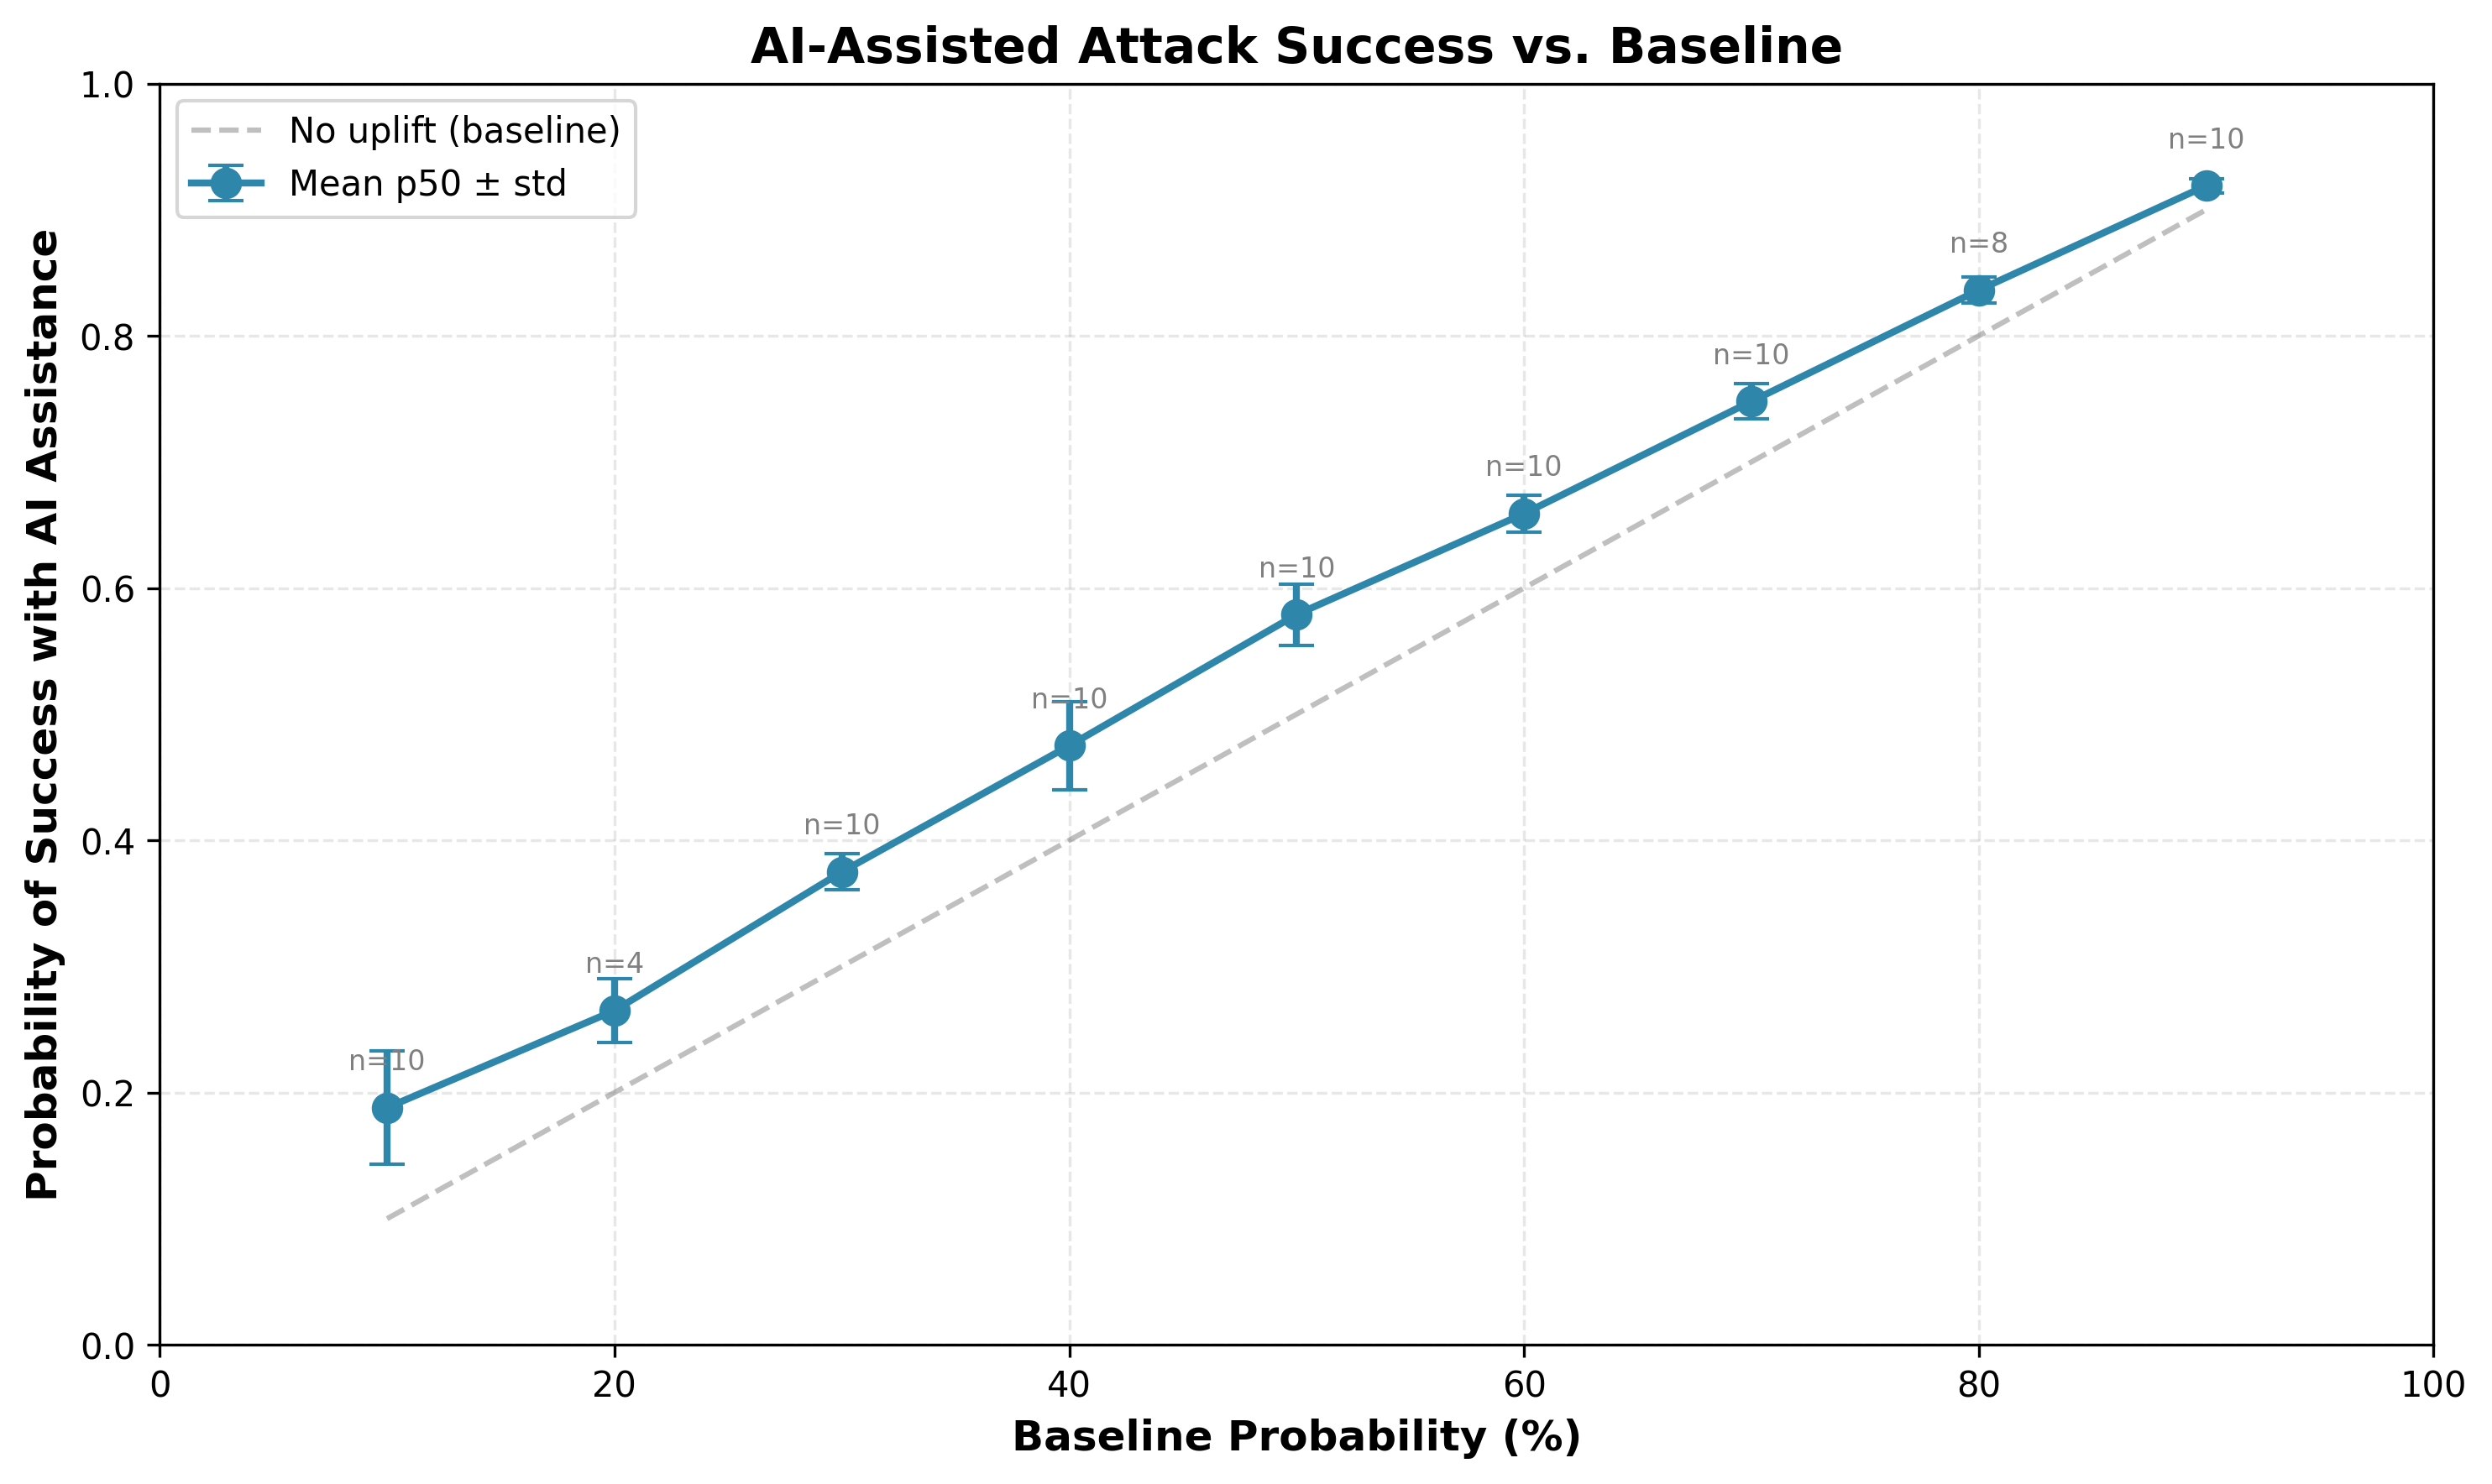
\includegraphics[width=0.7\textwidth]{figures/baseline_uplift_plot_week5.png}
  \caption{Median probability vs baseline (10--90\%), showing approximately linear relationship with ceiling effect. Error bars: IQR across 10 runs.}
  \label{fig:baseline_uplift}
\end{figure}

\begin{figure}[htbp]
  \centering
  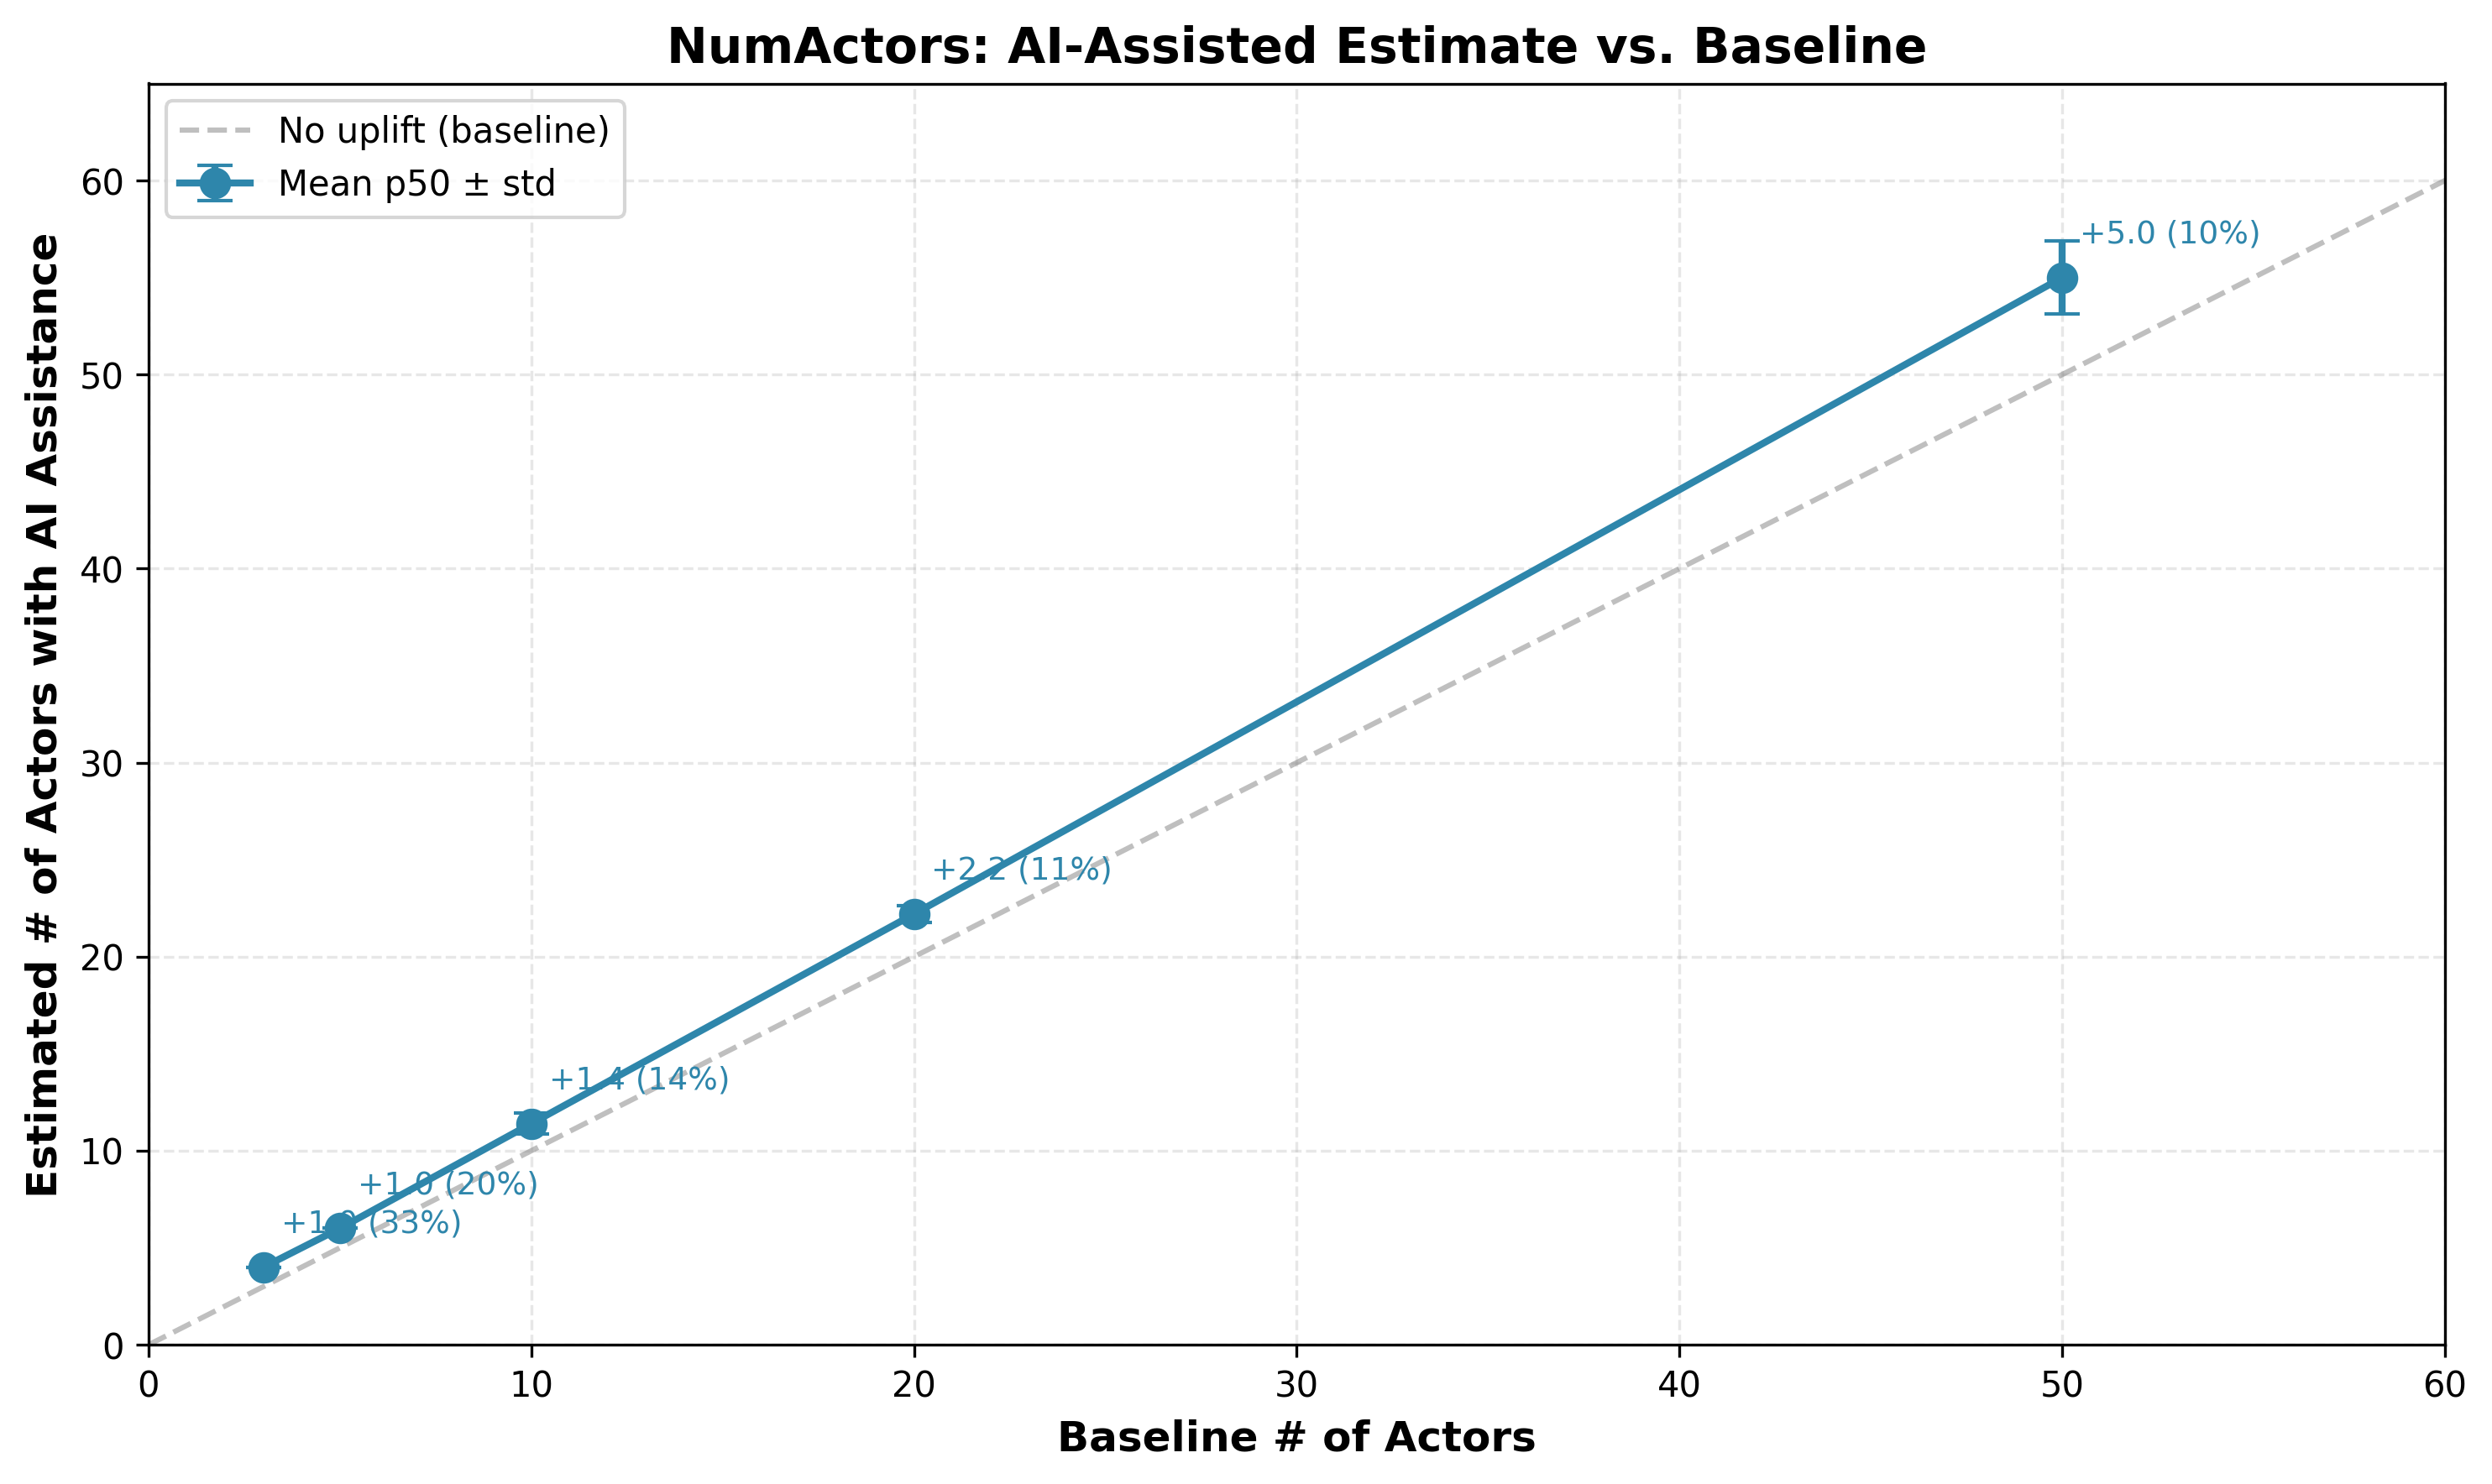
\includegraphics[width=0.7\textwidth]{figures/numactors_baseline_uplift_plot.png}
  \caption{Number of actors vs baseline shows linear relationship without ceiling effects (unbounded estimate).}
  \label{fig:numactors_uplift}
\end{figure}

\textbf{Prompt Component Sensitivity}

We tested seven prompt conditions (Claude Sonnet 4.5, single persona, TA0002 50\% baseline, Imaginairy, 10 runs per condition) measuring distributional shift via W$_1$ distance from full control prompt (615 words):

\begin{enumerate}
\item \textbf{Control:} Full prompt
\item \textbf{no\_ci:} Removed uncertainty range from baseline
\item \textbf{no\_baseline:} Removed point estimate from baseline
\item \textbf{no\_baseline\_no\_ci:} Removed entire baseline
\item \textbf{skip\_analysis:} Removed 4-section capability analysis
\item \textbf{trim\_reasoning:} Removed 3-phase reasoning scaffold
\item \textbf{trim\_all:} Removed analysis + reasoning + technical output ($\sim$100 words)
\end{enumerate}

\textit{Results} (Table~\ref{tab:prompt_sensitivity}, Figure~\ref{fig:prompt_sensitivity}): Baseline removal caused largest shifts (no\_baseline: W$_1$=0.154, 18.1$\times$ variance; no\_baseline\_no\_ci: W$_1$=0.230, 12.3$\times$ variance). Removing CI alone had minimal impact (W$_1$=0.013, 0.36$\times$ variance). Surprisingly, trimming reasoning/analysis reduced variance (trim\_reasoning: 0.30$\times$; trim\_all: 0.07$\times$) while maintaining similar central estimates, suggesting convergence under shorter prompts.

\begin{table}[htbp]
\centering
\caption{Prompt sensitivity: W$_1$ distance from control and variance multiplier.}
\label{tab:prompt_sensitivity}
\begin{tabular}{lcc}
\toprule
\textbf{Condition} & \textbf{W$_1$} & \textbf{Variance ($\times$Control)} \\
\midrule
Control (615 words) & --- & 1.00$\times$ \\
no\_ci & 0.013 & 0.36$\times$ \\
no\_baseline & 0.154 & 18.1$\times$ \\
no\_baseline\_no\_ci & 0.230 & 12.3$\times$ \\
skip\_analysis & 0.041 & 0.78$\times$ \\
trim\_reasoning & 0.011 & 0.30$\times$ \\
trim\_all ($\sim$100 words) & 0.016 & 0.07$\times$ \\
\bottomrule
\end{tabular}
\end{table}

\begin{figure}[htbp]
  \centering
  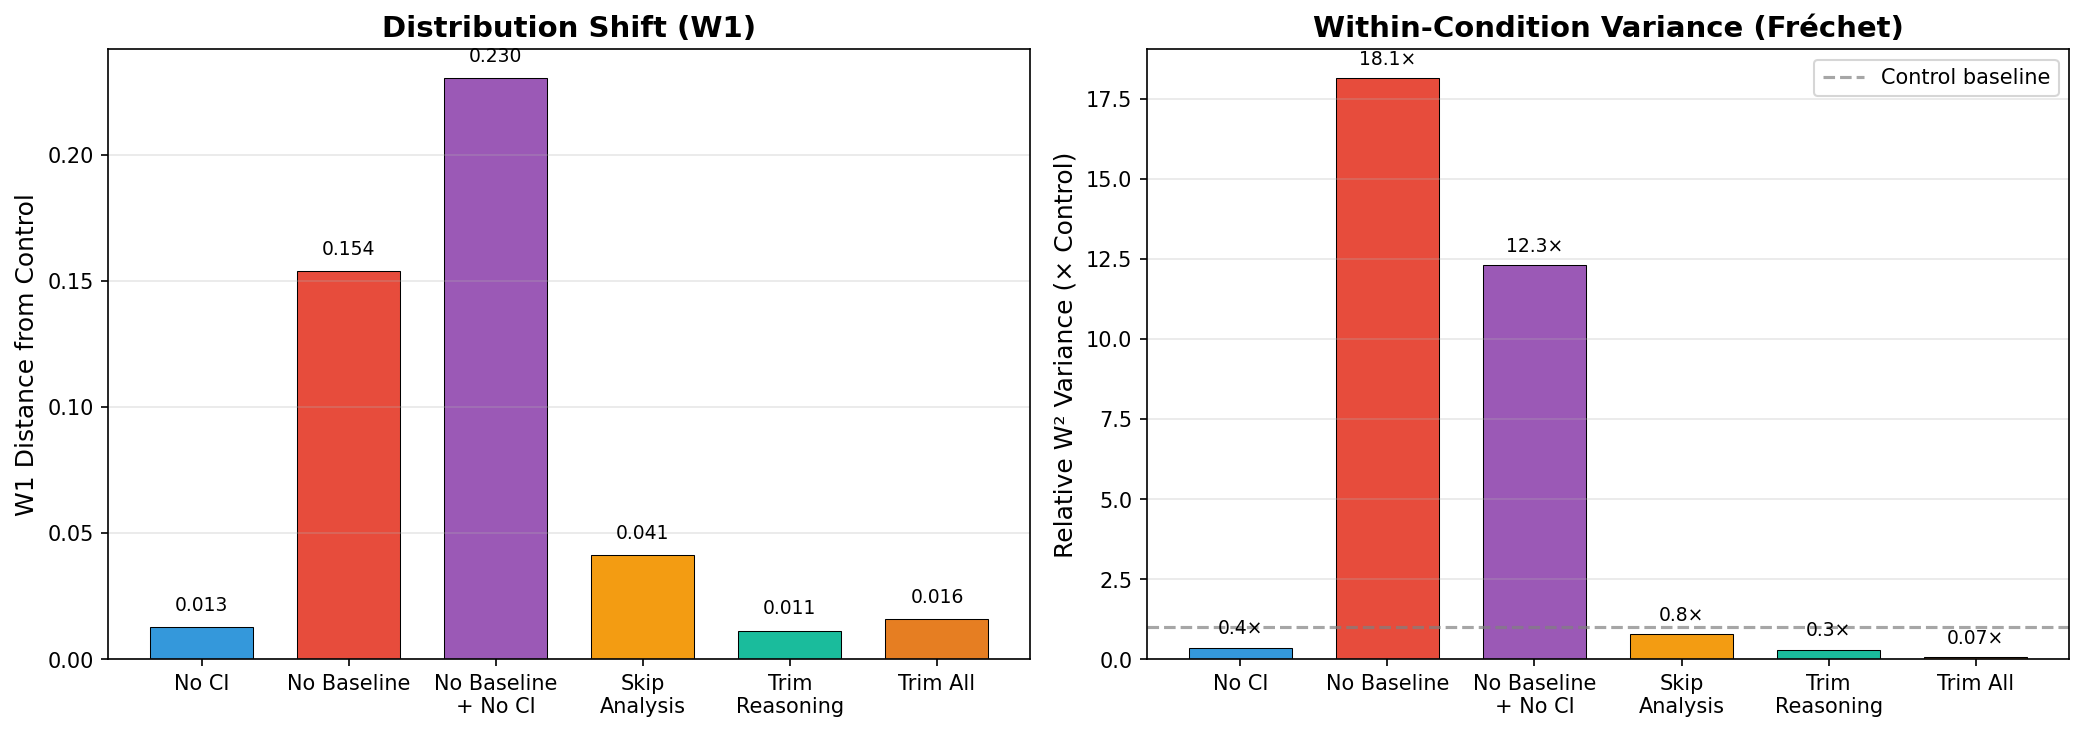
\includegraphics[width=0.75\textwidth]{figures/w1_chart (1)_week5.png}
  \caption{W$_1$ distance across seven prompt conditions. Baseline-removal shifts most; trimming reduces variance.}
  \label{fig:prompt_sensitivity}
\end{figure}
